\section{Benchmark Setting}
\label{sec:data}

\begin{figure}[H]
\centering
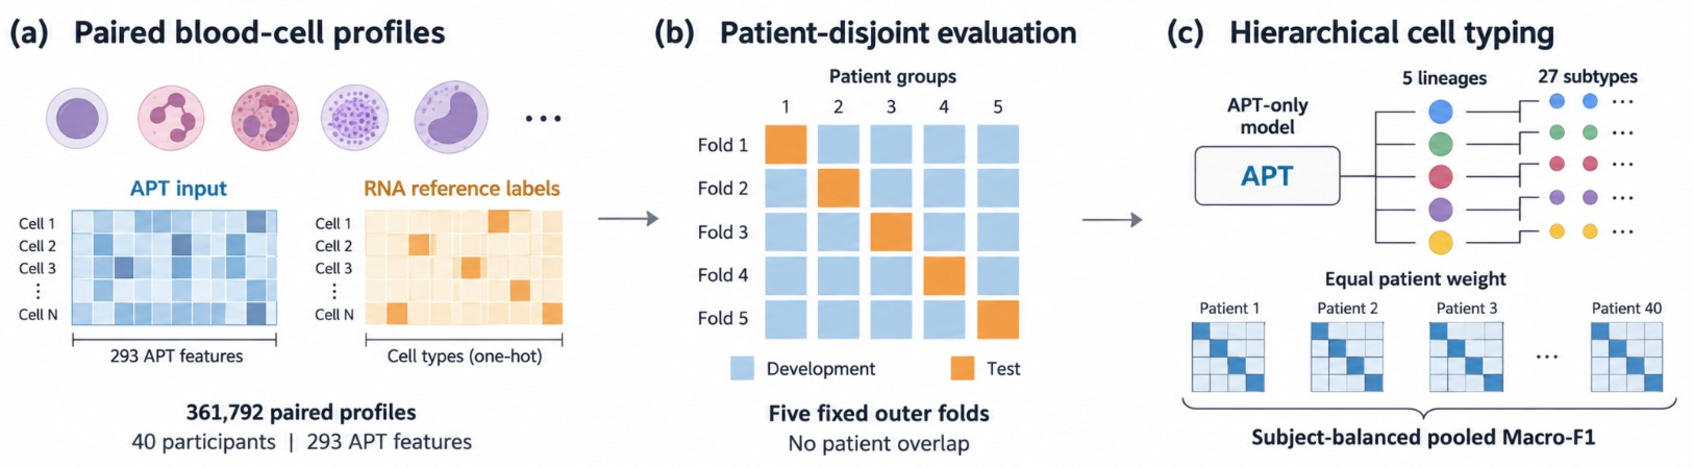
\includegraphics[width=\linewidth]{figures/cell_patient_overview.pdf}
\caption{The primary \ourbench{} contract. Patient-disjoint outer folds evaluate
cell typing in new individuals; subject-normalized confusion pooling assigns
equal total scoring weight to each patient.}
\label{fig:cell_patient_overview}
\end{figure}

\subsection{Blood Profiles and Reference Labels}
\label{sec:data:description}

\ourbench{} is derived from peripheral-blood specimens from \numparticipants{} participants in
five cancer groups (CRC, GC, HCC, PC, and BTC) and healthy controls, with 6--8
participants per group. The paired assay measures transcriptomic state and \numaptfeatures{}
aptamer features on the same cells. Transcriptomic counts
were processed with Seurat \citep{hao2021integrated}; predicted doublets and
low-quality cells were removed, and clusters were manually annotated using
canonical markers from prior PBMC and pan-cancer studies
\citep{mcginnis2019doubletfinder,zhang2024pan,yang2024pan}. These annotations
define \numlineages{} lineages and \numsubtypes{} subtypes. They are operational reference
labels, not independently measured biological truth.

The linked post-QC cohort contains 374{,}854 cells. Excluding the uncertain
\emph{Unknown} subtype leaves \numcells{} benchmark cells. Each subtype has one
fixed parent lineage. Disease is a six-class patient attribute, not the root of
the cell hierarchy: any given lineage can occur in multiple disease groups.
We evaluate the lineage-to-subtype hierarchy without imposing a
disease-to-lineage-to-subtype label tree. The construction checklist and
unresolved acquisition and annotation fields are recorded in
Appendix~\ref{sec:appendix:dataset_documentation}.

\subsection{Patient-Disjoint Cell-Typing Contract}
\label{sec:data:contract}
\label{sec:data:protocols}

The primary task is cell typing in new patients.
\textbf{Cell identity} predicts lineage and subtype using APT alone at inference.
Training supervision is recipe-specific: only Soft-cascade additionally uses
development-patient disease labels for contrastive pairing.
Open-set subtype discovery is outside the contract; all primary cell tasks
use the fixed five-lineage/27-subtype ontology.

\numfolds{} frozen disease-stratified folds each hold out eight patients. All cells
from a patient remain together. Benchmark-fitted transforms, model selection,
and fitting use development patients; the upstream provenance of the supplied
APT expression remains incompletely recovered
(Appendix~\ref{sec:appendix:main_protocols}). We pool predictions across the five
out-of-fold (OOF) partitions. The release
interface records cell and patient IDs, ontology, folds, predictions, and
metrics (Appendix~\ref{sec:appendix:benchmark_release}). Full data access and a
portable end-to-end evaluator remain release requirements.

\subsection{Metrics and Statistical Units}
\label{sec:data:imbalance}

Coarse and fine subject-balanced pooled Macro-F1 (SB-Macro-F1) are the primary
cell metrics. For patient $p$, let $C^{(p)}$ be the confusion matrix over a fixed
$K$-class ontology and $n_p$ its number of evaluated cells. Define
\begin{equation}
\overline C=\frac{1}{P}\sum_{p=1}^{P}\frac{C^{(p)}}{n_p},\qquad
\mathrm{SB\text{-}MacroF1}=\frac{1}{K}\sum_{k=1}^{K}
\frac{2\overline C_{kk}}{\sum_j\overline C_{kj}+\sum_i\overline C_{ik}}.
\label{eq:primary_sb_f1}
\end{equation}
A zero denominator contributes zero. Each patient's entire matrix, not each
class row, is normalized to unit mass. This differs from cell-weighted pooled
Macro-F1 and from mean within-subject Macro-F1. We retrospectively re-score the
frozen OOF predictions under this primary reporting convention; checkpoints
are not reselected.

Main-table intervals use 2{,}000 resamples and explicitly label their target:
P denotes patient uncertainty conditional on frozen fits, and SP additionally
resamples the three MLP training seeds. Each SP replicate averages three
seed-specific scores, using the same patient draw across them. Both are
pointwise and conditional on the fixed fold design; neither repeats model
selection. The comparison is descriptive, and an individual-score interval
is not a pairwise superiority test. Full resampling order is given in
Appendix~\ref{sec:appendix:identity_questions}.

The paired-RNA probe also uses subject-balanced pooled Macro-F1, but has a
different training budget and preprocessing protocol; its scores must not be
interpreted as additional architecture rows in the main table.
The experimental protocol is in Appendix~\ref{sec:appendix:identity_questions};
scoring-unit comparisons are in Appendix~\ref{sec:appendix:protocol_sensitivity}.
